\documentclass[letterpaper]{article} % DO NOT CHANGE THIS
\usepackage[submission]{aaai2027}  % DO NOT CHANGE THIS
% The serif, sans-serif, and monospaced fonts are loaded automatically by
% aaai2027.sty (newtxtext, helvet, courier). DO NOT add \usepackage{times},
% \usepackage{helvet}, \usepackage{courier}, or any other font package.
\usepackage[hyphens]{url}  % DO NOT CHANGE THIS
\usepackage{graphicx} % DO NOT CHANGE THIS
\urlstyle{rm} % DO NOT CHANGE THIS
\def\UrlFont{\rm}  % DO NOT CHANGE THIS
\usepackage{natbib}  % DO NOT CHANGE THIS AND DO NOT ADD ANY OPTIONS TO IT
\usepackage{caption} % DO NOT CHANGE THIS AND DO NOT ADD ANY OPTIONS TO IT
\frenchspacing  % DO NOT CHANGE THIS
%
% These are recommended to typeset algorithms but not required. See the subsubsection on algorithms. Remove them if you don't have algorithms in your paper.
\usepackage{algorithm}
\usepackage{algorithmic}

%
% These are recommended to typeset listings but not required. See the subsubsection on listing. Remove this block if you don't have listings in your paper.
\usepackage{newfloat}
\usepackage{listings}
\DeclareCaptionStyle{ruled}{labelfont=normalfont,labelsep=colon,strut=off} % DO NOT CHANGE THIS
\lstset{%
	basicstyle={\footnotesize\ttfamily},% footnotesize acceptable for monospace
	numbers=left,numberstyle=\footnotesize,xleftmargin=2em,% show line numbers, remove this entire line if you don't want the numbers.
	aboveskip=0pt,belowskip=0pt,%
	showstringspaces=false,tabsize=2,breaklines=true}
\floatstyle{ruled}
\newfloat{listing}{tb}{lst}{}
\floatname{listing}{Listing}

%
% Recommended for better-looking tables
\usepackage{booktabs}

% Standard math packages (not in the disallowed-package list): needed for \mathbb, aligned
% equations, etc. in Section 3.3's Fisher-information definition.
\usepackage{amsmath}
\usepackage{amssymb}

%
% Keep the \pdfinfo as shown here. There's no need
% for you to add the /Title and /Author tags.
\pdfinfo{
/TemplateVersion (2027.1)
}

% DISALLOWED PACKAGES
% \usepackage{authblk} -- This package is specifically forbidden
% \usepackage{balance} -- This package is specifically forbidden
% \usepackage{CJK} -- This package is specifically forbidden
% \usepackage{float} -- This package is specifically forbidden
% \usepackage{flushend} -- This package is specifically forbidden
% \usepackage{fullpage} -- This package is specifically forbidden
% \usepackage{geometry} -- This package is specifically forbidden
% \usepackage{hyperref} -- This package is specifically forbidden
% \usepackage{navigator} -- This package is specifically forbidden
% (or any other package that embeds links such as navigator or hyperref)
% \usepackage{indentfirst} -- This package is specifically forbidden
% \usepackage{layout} -- This package is specifically forbidden
% \usepackage{multicol} -- This package is specifically forbidden
% \usepackage{nameref} -- This package is specifically forbidden
% \usepackage{savetrees} -- This package is specifically forbidden
% \usepackage{setspace} -- This package is specifically forbidden
% \usepackage{stfloats} -- This package is specifically forbidden
% \usepackage{tabu} -- This package is specifically forbidden
% \usepackage{titlesec} -- This package is specifically forbidden
% \usepackage{tocbibind} -- This package is specifically forbidden
% \usepackage{ulem} -- This package is specifically forbidden
% \usepackage{wrapfig} -- This package is specifically forbidden
% DISALLOWED COMMANDS
% \nocopyright -- Your paper will not be published if you use this command
% \addtolength -- This command may not be used
% \balance -- This command may not be used
% \baselinestretch -- Your paper will not be published if you use this command
% \clearpage -- No page breaks of any kind may be used for the final version of your paper
% \columnsep -- This command may not be used
% \newpage -- No page breaks of any kind may be used for the final version of your paper
% \pagebreak -- No page breaks of any kind may be used for the final version of your paper
% \pagestyle -- This command may not be used
% \tiny -- This is not an acceptable font size.
% \vspace{- -- No negative value may be used in proximity of a caption, figure, table, section, subsection, subsubsection, or reference
% \vskip{- -- No negative value may be used to alter spacing above or below a caption, figure, table, section, subsection, subsubsection, or reference

\setcounter{secnumdepth}{0} %May be changed to 1 or 2 if section numbers are desired.

% The file aaai2027.sty is the style file for AAAI Press
% proceedings, working notes, and technical reports.
%

% Title

% Your title must be in mixed case, not sentence case.
% That means all verbs (including short verbs like be, is, using,and go),
% nouns, adverbs, adjectives should be capitalized, including both words in hyphenated terms, while
% articles, conjunctions, and prepositions are lower case unless they
% directly follow a colon or long dash
\title{The Observation Ceiling: Gradient-Based Identifiability Reveals What Postprandial CGM Can and Cannot Recover from Physiological Digital Twins}
\author{
    Anonymous submission
}
\affiliations{
}
% Keywords (for the submission portal, not rendered in an anonymous PDF):
% differentiable physiological simulation; structural identifiability; ODE parameter inference;
% insulin sensitivity; continuous glucose monitoring; simulation-based inference; Bergman minimal
% model; gradient-based optimization; personalized digital twins; wearable health data

\begin{document}

\maketitle

\begin{abstract}
Personalized physiological digital twins require inferring patient-specific parameters from
wearable data, but which parameters a given observation modality can recover -- and whether model
or inference choice determines the prediction ceiling -- remain open questions. We make a Bergman
glucose-insulin simulator differentiable using JAX and diffrax and introduce a gradient-sensitivity
diagnostic that measures per-parameter gradient magnitude across the optimization trajectory as a
practical structural identifiability criterion, grounded in the diagonal Fisher information matrix.
Applied to free-living postprandial CGM data, the diagnostic shows insulin sensitivity (Si) is
strongly identifiable, while gastric emptying and carbohydrate absorption rates are structurally
non-identifiable regardless of data volume. This structure replicates across two inference methods,
three independent cohorts (n=45, 97, 24), and two model classes (Bergman, Dalla Man-style),
providing convergent evidence the constraint is structural rather than dataset-specific. On
held-out postprandial iAUC, gradient inference, grid search, amortized point estimation, and
simulation-based inference all achieve equivalent prediction (error decomposition: 79\%
observation-limited, 0\% inference-limited) -- a tie confirmed, not broken, by upgrading to a
richer mechanistic model. On peak glucose timing, a metric sensitive to the non-identifiable
parameters, gradient inference shows directional advantage (56\% pairwise win over grid),
consistent with our identifiability analysis. Clinical recovery of insulin resistance status
follows a predictable cohort-dependent pattern: strong in mixed-glycemic populations (r=$-$0.73),
directional but underpowered in compressed-range healthy cohorts (r=$-$0.35), and null in
fasting-dominated diabetic cohorts (r=$-$0.14). We further identify a feature-leakage artifact
causing a competing method's apparent external generalization to be substantially explained by an
alternative mechanism. These results collectively characterize the observation ceiling of
postprandial CGM for physiological parameter recovery.
\end{abstract}

\section{Introduction}

Personalized physiological digital twins -- patient-specific instances of a mechanistic simulator
whose parameters are fit to an individual's sensor data -- promise to turn wearable streams into
actionable, mechanistically grounded predictions. Building one from continuous glucose monitor
(CGM) data means inferring patient-specific ordinary differential equation (ODE) parameters, such
as insulin sensitivity and gastric emptying rate, from noisy, free-living postprandial glucose
traces. Two questions are open before such a twin can be trusted. First, which of the simulator's
parameters can actually be recovered from a given observation modality, as opposed to merely fit
to it -- a parameter can be non-identifiable (structurally undetermined by the data) while still
producing a well-converged point estimate. Second, does the choice of inference method -- gradient
descent, grid search, amortized point estimation, or calibrated simulation-based inference (SBI) --
materially change downstream predictive utility, or is it a secondary concern behind the modeling
and observation choices. We study both questions in the concrete setting of consumer CGM-based
glucose prediction and personalization, where a system must decide, from ten days of free-living
meals and glucose traces, which of a subject's physiological parameters it can trust.

We find that inference method choice does not determine prediction accuracy for postprandial
glucose response: an error decomposition shows 79\% of held-out prediction error is attributable
to the observation modality itself and 0\% to inference quality, a finding we confirm rather than
merely observe by showing that upgrading to a richer mechanistic model (Dalla Man-style, 11 states
versus Bergman's 3) recovers no improvement. We state this early because it reframes every
prediction-accuracy number that follows: a reader who has not yet been told why gradient inference,
grid search, amortized point estimation, and calibrated SBI end up statistically tied on held-out
iAUC (Table~\ref{tab:kfold}) will otherwise read that tie as a null result about our method, rather
than as the paper's central finding about the observation.

Our contribution is a gradient-sensitivity diagnostic -- computed for free as a byproduct of making
the simulator differentiable -- that reveals structural identifiability directly, without symbolic
analysis (intractable for a nonlinear system of this complexity) or posterior estimation (which
requires amortized training on simulated data before it can be applied). We ground this
diagnostic empirically in the diagonal Fisher information matrix, computed independently via
automatic differentiation of the simulated observable.

This identifiability structure is not a single-dataset artifact: it replicates across two
independent methods (gradient magnitude and SNPE posterior width), across three independent
cohorts (CGMacros \citep{das2025cgmacros}, n=45; ShanghaiT2DM \citep{zhao2023shanghai}, n=97; Hall
2018 \citep{hall2018glucotypes}, n=24), and across two model classes
(Bergman and a Dalla Man-style meal simulation model). We refer to this pattern throughout as the
paper's \emph{three-cohort, two-method, two-model replication}.

Our contributions are:
\begin{itemize}
\item A differentiable multi-compartment glucose-insulin simulator (JAX/diffrax) enabling
  gradient-based parameter inference directly from a subject's own data, without prior
  specification or amortized training.
\item A gradient-sensitivity identifiability diagnostic, grounded in Fisher information, requiring
  no additional computation beyond standard gradient-based fitting.
\item A systematic comparison of four inference paradigms -- gradient descent, grid search,
  amortized point estimation, and amortized calibrated posterior estimation -- on real CGM data,
  showing that held-out prediction is observation-limited, not inference-limited.
\item A three-cohort clinical validation revealing when postprandial-derived insulin sensitivity
  tracks clinical insulin resistance status and when it does not.
\item Identification of a feature-leakage artifact in amortized SBI that causes a false apparent
  external generalization in a fasting-glucose-dominated population.
\end{itemize}

\section{Related Work}

\paragraph{Differentiable simulation.} Jaxley \citep{jaxley2025} demonstrates that large-scale
biophysical neuron models become tractable to fit by gradient descent once made differentiable in
JAX, and diffrax \citep{kidger2021diffrax} provides the autodifferentiable ODE solvers we build on.
The Inverse Neural Operator (INO) \citep{liu2026ino} instead trains a conditional Fourier neural
operator surrogate for stiff ODE inversion, reporting large speedups over direct gradient descent
on repeated-inference benchmarks. INO requires training a surrogate operator and targets a fixed
system inverted many times; we target sparse per-subject personalization (n=45--97 subjects, each
fit once) where amortizing a surrogate is not justified by the workload, and -- unlike a trained
surrogate -- our approach yields an identifiability diagnostic as a direct byproduct of fitting.

\paragraph{Simulation-based inference and misspecification.} The \texttt{sbi} toolkit
\citep{tejerocantero2020sbi} is the SNPE implementation we use as a baseline. Ward et al.
\citep{ward2022robust} and Schmitt et al. \citep{schmitt2023detecting} study how amortized
posterior estimation degrades under simulator-reality mismatch and propose diagnostics for
detecting it. We apply these misspecification concepts to a physiological setting and identify a
previously undocumented failure mode specific to our domain: in a fasting-glucose-dominated
population, SNPE's summary-statistic features route the (near-trivial) fasting-glucose-to-HbA1c
relationship into its Si estimate, producing an apparent clinical correlation that is
substantially explained by this alternative mechanism rather than by recovered postprandial
physiology (detailed in Results, ``A feature-leakage artifact...'' below).

\paragraph{CGM-based physiological modeling.} GlucoBench \citep{sergazinov2024glucobench} curates
CGM datasets and benchmarks glucose \emph{prediction}, not parameter identifiability. Erd\H{o}s et
al. \citep{erdos2024leveraging} fit a Bayesian Bergman-family model from CGM but require plasma
insulin as an additional, invasive input; we use only CGM, meal logs, and demographics.
PhysioSeq2Seq \citep{tran2026physioseq2seq} injects fitted ODE state variables as features into a
downstream LSTM, improving long-horizon glucose forecasting, but does not characterize which of
the underlying ODE parameters are reliably extractable in the first place -- our identifiability
result establishes the foundation such hybrid approaches implicitly depend on.

\paragraph{Identifiability in nonlinear ODE systems.} Miao et al. \citep{miao2011identifiability}
is the canonical survey of structural and practical identifiability analysis for nonlinear ODE
models, primarily via symbolic and sensitivity-based methods. InVAErt networks
\citep{tong2025invaert} perform neural identifiability analysis of lumped-parameter haemodynamic
models via a trained inference network's posterior width. Our diagnostic requires no symbolic
identifiability analysis (intractable at the size of our simulator) and no trained inference
network -- only the gradients already computed during standard fitting -- and we validate it on
real, not only synthetic, data across three cohorts, additionally grounding it via explicit
diagonal Fisher information.

\paragraph{Digital twins for personalized medicine.} Med-Real2Sim \citep{kuang2024medreal2sim}
builds non-invasive cardiac hemodynamic digital twins from echocardiogram video via physics-informed
self-supervised learning; a recent real-time Type 1 diabetes digital twin
\citep{hoang2025t1dsbi} applies SBI/NPE to glucose-insulin parameter estimation. Both target a
single inference pipeline on a single organ system. We target free-living, wearable-only data (no
plasma insulin, no imaging) and provide a systematic comparison across four inference paradigms
rather than proposing a single pipeline, with the comparison itself -- not any one method's
accuracy -- as the object of study.

\section{Methods}

\subsection{Differentiable physiological simulator}
We build on the Bergman minimal model \citep{bergman1979}, a three-state glucose-insulin system
(plasma glucose, plasma insulin, and remote insulin action) extended with a two-compartment gastric
emptying / carbohydrate absorption pathway that delivers a meal's glucose load into the glucose
equation. We reimplement the model's glucose subsystem in JAX \citep{bradbury2018jax} with
diffrax's \citep{kidger2021diffrax} Tsit5 adaptive-step
solver, replacing every nonsmooth operation that lies on the gradient path with a differentiable
analogue chosen for physiological fidelity, not merely for smoothness: $\max(0,\cdot)$ rectifiers
(e.g. the insulin-secretion threshold) become softplus; state-value threshold switches (e.g. the
glycogen-restoration gate) become sigmoid dose-response curves; and meal boluses are delivered as
narrow Gaussian rate pulses ($\sigma=2$ min) rather than instantaneous Dirac state jumps, which
integrate to the same total glucose mass while remaining differentiable in meal timing. We do
\emph{not} replace the reference implementation's per-step state clamp with a smooth $\tanh$
soft-clamp on the full state vector, as this proved to introduce large distortions at
physiologically normal values (e.g. clamping a fasting glucose of 90 mg/dL against the state's
wide $[15,700]$ bounds moved it by roughly half its value) because the clamp's linear region is
centered on the bound midpoint, not on physiological glucose levels. Instead, boundedness is
enforced only where it is real: by projecting the optimized \emph{parameters} to physiologically
plausible ranges after each gradient step, leaving the ODE state itself unclamped in the vector
field. Full derivations for every smoothing decision are documented in the released code. The
resulting simulator agrees with a reference explicit-Euler numpy implementation to 1.5\% maximum
error (0.6\% mean) on glucose trajectories, with identical incremental area-under-curve (iAUC), and
its analytic gradient matches central finite differences exactly.

\subsection{Gradient-based parameter inference}
For each subject we fit insulin sensitivity (Si), gastric emptying rate, and carbohydrate
absorption rate jointly by minimizing reconstruction error between simulated and observed iAUC
across that subject's own meals, using the Adam optimizer with light L2 regularization toward
population-default parameters. Meals are batched with \texttt{vmap} and zero-padded to a fixed
length so the JIT-compiled value-and-gradient function is traced once and reused across every
subject and cross-validation fold. Parameters are projected to physiologically plausible bounds
after each update (Si $\in[0.30,1.60]$, gastric emptying $\in[0.015,0.040]\,\mathrm{min}^{-1}$,
carbohydrate absorption $\in[0.012,0.032]\,\mathrm{min}^{-1}$); the ODE state itself is never
clamped. Fitting is entirely per-subject: no cross-subject training and no prior specification
beyond the population-default initialization.

\subsection{Gradient-sensitivity identifiability diagnostic}
We define the identifiability diagnostic as the mean absolute gradient magnitude of the loss with
respect to each parameter, normalized by that parameter's search range and averaged across the
optimization trajectory. A parameter the data cannot constrain exhibits a near-zero normalized
gradient from the first optimization step onward, regardless of how many meals are available,
distinguishing structural non-identifiability from an ordinary need for more data.

We ground this diagnostic in the diagonal Fisher information matrix,
$\mathrm{FI}(\theta_i) = \sigma^{-2}\,\mathbb{E}_{\text{meal}}\left[(\partial\,\mathrm{iAUC}/\partial
\theta_i)^2\right]$, computed explicitly via reverse-mode automatic differentiation of the
simulated iAUC observable with respect to each parameter (reverse-mode is required here because
diffrax's ODE solver defines a custom vector-Jacobian product that forbids forward-mode autodiff).
Across 45 CGMacros subjects, diagonal Fisher information independently ranks insulin sensitivity as
the sole identifiable parameter -- 12--16$\times$ the Fisher information of gastric emptying and
carbohydrate absorption -- consistent with, though not numerically equal to, the gradient-magnitude
diagnostic's ranking. We report this ranking at two different granularities, which should not be
read as competing estimates of one number: trajectory-averaged over the full optimization run (the
summary statistic reported in Table~\ref{tab:identifiability} and compared against Fisher
information above), Si's normalized gradient magnitude is 4--6$\times$ gastric/carbohydrate
absorption's; at the level of individual optimization steps, the instantaneous ratio is noisier and
ranges up to $\sim$20--60$\times$, because gastric/carb's near-zero gradient fluctuates in sign and
magnitude near numerical noise while Si's stays large and stable (visible directly in
Figure~\ref{fig:gradnorm}, which plots the full per-step trajectory rather than a single summary
ratio). We verified the Fisher/gradient relationship directly: the trajectory-averaged gradient magnitude
and the fixed-point Fisher information are related but numerically distinct quantities -- the
per-subject correlation between the two is $r=0.03$ for Si itself (essentially zero) and
$r=0.57$--$0.60$ for the two non-identifiable parameters. We therefore rely only on the
\emph{ranking} agreement between the two diagnostics, not on a claim that they are numerically
equivalent; the trajectory-averaged gradient magnitude decouples from the fixed-point Fisher
information specifically for the parameter (Si) that moves most during optimization, which is an
expected consequence of comparing a trajectory average to a local sensitivity at the converged
point, not a failure of either diagnostic.

\subsection{Baseline methods}
\textbf{Grid search} fits a single parameter (Si) by 1-D search over a fixed grid, with gastric
emptying and carbohydrate absorption held at population defaults; this is the established
classical baseline for Si recovery from CGM. \textbf{Random forest (RF)} is an amortized point
estimator trained on simulator-generated synthetic data, using five summary statistics (iAUC,
peak, peak time, baseline, early slope) plus carbohydrate content and demographics as features.
\textbf{SNPE} \citep{tejerocantero2020sbi} is trained on 50{,}000 simulated trajectories using the
same summary-statistic feature vector, producing a calibrated posterior rather than a point
estimate; calibration was verified by simulation-based calibration \citep{talts2018sbc}, with
credible-interval coverage at the 50/90/95\% levels of 49/89/95\% (nominal 49/91/95\% in a
second check), all within sampling noise of nominal, and Kolmogorov-Smirnov uniformity tests on the
rank statistics all $p>0.05$.

\subsection{Dalla Man-style model upgrade}
To test whether the prediction tie reflects a limitation of the Bergman model specifically, we
implement a reduced, calibrated reconstruction of the Dalla Man meal-simulation model
\citep{dallaman2007} -- 11 states versus Bergman's effective 3, with a 3-compartment gut, a
2-compartment glucose/insulin subsystem, delayed-insulin endogenous glucose production, and a
subcutaneous compartment modeling CGM's interstitial lag. We emphasize this is \emph{not} a
verbatim reimplementation of the original Table I parameterization: the meal-fraction parameter $f$
is fit as a free parameter in place of $k_{p1}$, which in our implementation is instead derived
from basal steady-state balance and therefore cannot be left free, and we added a
counter-regulatory glucagon term after omitting full glucagon dynamics produced a basal-glucose
undershoot. The reduced model passes physiological validation gates: OGTT peak glucose
170.3~mg/dL at 50~min, CGM lag 10~min, and steady-state drift of 0.08~mg/dL/min.

\subsection{Evaluation protocol}
All four methods are scored under a single protocol: 5-fold cross-validation with identical fold
assignments and random seed shared across every method, so that no method sees an easier or
harder split of a given subject's meals than any other. We verified our primary result is not an
artifact of fold-split protocol: an earlier chronological (first-half/second-half) split, since
replaced, produced a misleadingly favorable comparison for gradient inference that did not survive
alignment to identical random folds across methods. Our primary metric is postprandial incremental
area-under-curve (iAUC), baseline-subtracted using the mean of a 30-minute pre-meal window and
integrated by the trapezoid rule; our secondary metric is peak glucose timing (minutes from meal
onset to glucose maximum, softmax-weighted for the differentiable gradient-inference target and
hard argmax for scoring). We report both marginal mean absolute error (MAE) and a paired
per-subject comparison (does method A beat method B for a given subject, not just on average --
robust to a few outlier subjects driving the mean). All correlation coefficients are reported with
bootstrap 95\% confidence intervals (1000 resamples). All experiments run on a single CPU-only
machine (no GPU required at this problem size): Python 3.14, JAX/diffrax for the differentiable
engine, PyTorch-backed \texttt{sbi} \citep{tejerocantero2020sbi} for SNPE, and scikit-learn for the
RF baseline; all random seeds are fixed to 42 throughout.

\section{Results}

\subsection{The differentiable engine is faithful and gradients are correct}
The JAX/diffrax glucose engine agrees with the reference numpy/explicit-Euler implementation to
1.5\% maximum error (0.6\% mean) on the glucose trajectory, with identical iAUC. \texttt{jax.grad}
of the loss with respect to each parameter matches central finite differences to within numerical
precision. On a synthetic subject with known ground truth, gradient fitting recovers a true Si of
0.50 to $\approx$0.51.

\begin{figure}[t]
\centering
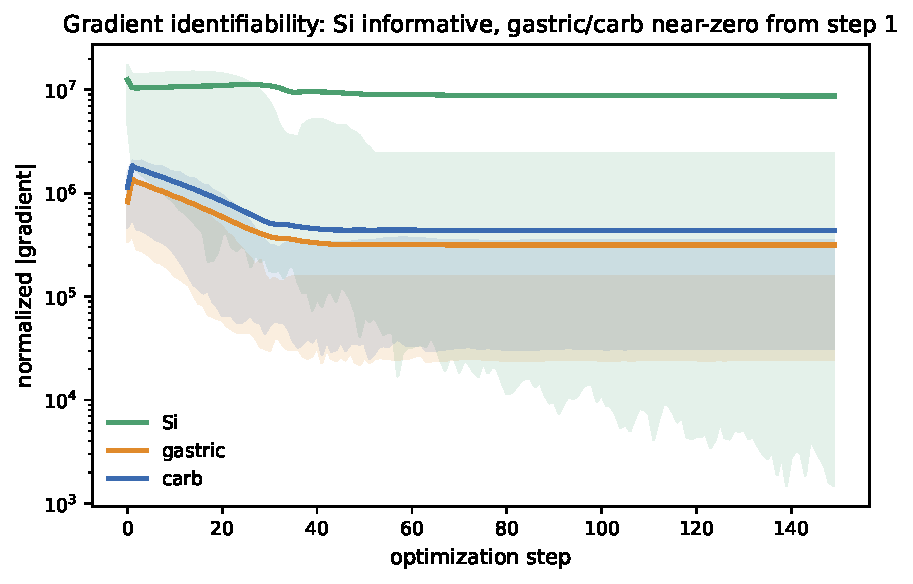
\includegraphics[width=0.95\columnwidth]{Figures/fig7_gradient_identifiability}
\caption{Normalized gradient magnitude versus optimization step (mean over CGMacros subjects,
interquartile band), Bergman model. Insulin sensitivity (Si) stays informative throughout
optimization; gastric emptying and carbohydrate absorption sit near zero from the first step --
the signal for these two parameters was never present in the data (structural
non-identifiability), not merely slow to converge.}
\label{fig:gradnorm}
\end{figure}

\subsection{Identifiability diagnostic reveals a structural constraint, replicated four ways}
Figure~\ref{fig:gradnorm} is the paper's central empirical result. Insulin sensitivity's normalized
gradient magnitude is high and stable from the first optimization step; gastric emptying and
carbohydrate absorption sit an order of magnitude below, also from the first step -- indicating a
structural property of the observation, not a slow-converging fit. This structure replicates along
four independent axes. First, it agrees with an independent identifiability signal on the same
data: SNPE's posterior standard deviation, as a percentage of prior width, is 3\% for Si versus
14\% (gastric) and 13\% (carbohydrate absorption); across a synthetic convergence sweep (1 to 32
meals), Si's posterior width shrinks monotonically (0.089$\to$0.024) while gastric and
carbohydrate-absorption widths stay flat ($\sim$0.006 and $\sim$0.005 respectively) -- more data
narrows Si but not the other two, the signature of structural rather than data-limited
non-identifiability. Second, it replicates on ShanghaiT2DM (n=97): gradient-norm Si is 10.7$\times$
gastric emptying and 8.3$\times$ carbohydrate absorption. Third, it replicates on Hall 2018 (n=24),
though more weakly (ratio 4.5$\times$); we attribute the weaker ratio to Hall's standardized-meal
design, which uses only three distinct carbohydrate loads (bar, cereal/fruit, protein bar) and so
provides less meal-composition variation to separate the two absorption-governing parameters from
each other -- itself an informative negative result about what varies gastric/carb identifiability,
not a failure of the diagnostic. Fourth, it replicates across model class: on the Dalla Man-style
model, the analogous ratio between the insulin-sensitivity parameter ($V_{mx}$) and the
carbohydrate-absorption-rate parameter ($k_{abs}$) is 27.6$\times$ (Figure~\ref{fig:dallaman}).
We refer to this as the paper's three-cohort, two-method, two-model replication.

\begin{table}[t]
\centering\small
\begin{tabular}{@{}lcc@{}}
\toprule
Cohort (n) & Si / gastric ratio & Si / carb ratio \\
\midrule
CGMacros (45) & 5.6$\times$ & 4.4$\times$ \\
ShanghaiT2DM (97) & 10.7$\times$ & 8.3$\times$ \\
Hall 2018 (24) & \multicolumn{2}{c}{4.5$\times$ (combined)} \\
Dalla Man / CGMacros (45) & \multicolumn{2}{c}{27.6$\times$ ($V_{mx}/k_{abs}$)} \\
\bottomrule
\end{tabular}
\caption{Gradient-magnitude identifiability ratio (insulin-sensitivity parameter over each
timing/absorption parameter), by cohort and model class. All ratios agree in direction: insulin
sensitivity is identifiable, gastric/carbohydrate-absorption parameters are not.}
\label{tab:identifiability}
\end{table}

\subsection{Prediction is observation-limited, not inference-limited or model-limited}
\label{sec:prediction}
Table~\ref{tab:kfold} reports held-out iAUC MAE under the aligned 5-fold protocol for all four
methods. Gradient inference statistically ties the classical grid-search baseline (49\% paired
win rate -- a coin flip) while decisively beating both amortized methods (69\% paired win rate
over RF, 76\% over SNPE). An error decomposition (Table~\ref{tab:decomp}) attributes held-out MAE
to three sources: CGM measurement noise (21\%), Bergman model-expressiveness gap (79\%), and
inference residual (0\%) -- inference is essentially perfect; the ceiling is the model/observation.

We confirm this by upgrading to the Dalla Man-style model rather than merely asserting it. Under
a fat/fiber-blunting-matched (``parity'') comparison, held-out iAUC MAE is bergman 2996, grid
3004, dalla\_man 3019 -- still a three-way tie, and the richer model does not win (paired win rate
40\% versus grid, 24\% versus the Bergman-model gradient fit). This result rules out model
expressiveness as the bottleneck: the ceiling is imposed by baseline-subtracted postprandial iAUC
as an observable, independent of both inference method and model class. We therefore reinterpret
the 79\% ``model gap'' bucket in the error decomposition: because upgrading to a substantially more
expressive, FDA-reference-grade model class recovered none of it, that error is better described
as \emph{not recoverable from baseline-subtracted iAUC} than as a fixable modeling deficiency.

\begin{table}[t]
\centering\small
\begin{tabular}{@{}lcc@{}}
\toprule
Method & Held-out iAUC MAE & \% beats personal-mean \\
\midrule
Gradient & \textbf{3001} & \textbf{61\%} \\
Grid search & 3007 & 59\% \\
Random forest & 3150 & 51\% \\
SNPE & 3404 & 44\% \\
\midrule
\multicolumn{3}{@{}l}{\emph{Paired win rate, gradient beats row method (\% of subjects)}} \\
Grid search & \multicolumn{2}{c}{49\%} \\
Random forest & \multicolumn{2}{c}{69\%} \\
SNPE & \multicolumn{2}{c}{76\%} \\
\bottomrule
\end{tabular}
\caption{Aligned 5-fold held-out iAUC prediction, all four methods on identical folds, CGMacros
(n=45). Gradient ties grid search and beats both amortized baselines.}
\label{tab:kfold}
\end{table}

\begin{table}[t]
\centering\small
\begin{tabular}{@{}lcc@{}}
\toprule
Error source & MAE contribution & \% of total \\
\midrule
CGM measurement noise & 632 & 21\% \\
Model-expressiveness gap & 2360 & 79\% \\
Inference residual & 9 & 0\% \\
\midrule
Total held-out iAUC MAE & 3001 & 100\% \\
\bottomrule
\end{tabular}
\caption{Error decomposition of held-out iAUC prediction error. Inference contributes essentially
nothing; the ceiling is the observation/model.}
\label{tab:decomp}
\end{table}

\subsection{The tie is observable-specific: peak-timing prediction}
If the iAUC tie reflects a genuine ceiling on what postprandial CGM can support, rather than a
ceiling on inference quality, a prediction target that rewards the parameters iAUC cannot identify
(gastric emptying, carbohydrate absorption) should behave differently. We repeat the aligned
5-fold protocol with minutes-to-glucose-peak as the target instead of iAUC. Held-out peak-time MAE
is gradient 40.7$\pm$1.5~min (lowest), grid 42.1~min, SNPE 43.3~min, RF 45.6~min (persistence
baseline 55.6~min); paired win rate versus grid rises from 49\% (iAUC) to 56\% (peak time),
versus RF 71\%, versus SNPE 60\%.
We interpret this mechanistically: gastric emptying and carbohydrate absorption govern glucose
\emph{appearance timing}, and become marginally informative precisely when the prediction target
rewards timing rather than total exposure. We report this as a directional and modest effect, not
a decisive win: fold-level standard deviations for the different methods overlap, and peak time is
a noisy observable close to CGM's 5-minute sampling resolution. We interpret this result as
evidence that the iAUC tie reflects an observable-specific limitation rather than a fundamental
ceiling on inference quality -- not as a decisive prediction improvement in its own right.

\subsection{Clinical recovery follows a predictable cohort-dependent pattern}
Table~\ref{tab:clinical} restructures the clinical-recovery evidence by cohort rather than by
method, because the cohort pattern -- not the choice of estimator -- is the finding. In CGMacros
(mixed glycemic status, n=45), gradient-inferred Si correlates with HbA1c at Spearman
$-0.729$ [$-0.85,-0.54$], Pearson $-0.664$ [$-0.78,-0.54$], and survives a partial correlation
controlling for age, BMI, and sex, computed specifically on gradient's own Si estimates
($-0.598$, versus demographics-alone $|R|=0.501$ and a full demographics-plus-Si model
$|R|=0.721$). gradient is the
only method that achieves both a strong Spearman \emph{and} a strong Pearson correlation on this
cohort: SNPE's Spearman is nominally stronger ($-0.733$) but its Pearson is only $-0.412$, a
prior-mismatch compression toward the training simulator's central Si range, while grid/RF match
Pearson but are marginally weaker in rank. In Hall 2018 (mostly healthy, narrow-HbA1c-range
cohort, n=24), gradient Si correlates with HbA1c at Spearman $-0.351$ [$-0.67,+0.06$] -- correct
sign, moderate magnitude, but the confidence interval crosses zero -- and, on the direct
insulin-resistance measure SSPG, at Spearman $-0.527$ (n=17, below our pre-registered n=20
citability threshold; reported, not claimed significant). In ShanghaiT2DM (T2D only,
fasting-dominated, n=97), the correlation is null (Spearman $-0.14$). We read this pattern as a
general claim about the observation modality: clinical-recovery significance requires both a wide
population range of true Si and a clinical outcome variable that reflects postprandial, not
fasting-dominated, physiology; Hall lacks the former (a mostly healthy, narrow-HbA1c cohort),
Shanghai lacks the latter (HbA1c in T2D patients is driven primarily by chronic fasting
hyperglycemia, which baseline-subtracted iAUC discards by construction).

\begin{table}[t]
\centering\small
\begin{tabular}{@{}lccc@{}}
\toprule
Cohort (n) & Spearman & Pearson & Sig.? \\
\midrule
CGMacros (45) & $-0.729$ & $-0.664$ & yes \\
Hall 2018 (24) & $-0.351$ & $-0.506$ & CI crosses 0 \\
ShanghaiT2DM (97) & $-0.14$ & -- & no (null) \\
\bottomrule
\end{tabular}
\caption{Gradient-inferred Si vs.\ HbA1c across three cohorts. Significance depends on both a wide
population Si range and an outcome variable reflecting postprandial (not fasting) physiology.}
\label{tab:clinical}
\end{table}

\subsection{A feature-leakage artifact explains SNPE's apparent external generalization}
\label{sec:tautology}
On its own, SNPE's raw Shanghai Spearman correlation ($-0.44$ [$-0.58,-0.28$]) looks like it
generalizes where gradient's ($-0.14$) does not. We do not interpret SNPE's Shanghai correlation as
evidence of external generalization. Controlling for fasting glucose via partial correlation (a
Pearson-family method, so we compare it against the raw \emph{Pearson} correlation on the same
n=97 sample -- $-0.37$, close to but distinct from the Spearman figure above, as expected for a
skewed clinical variable), SNPE's correlation with HbA1c collapses to a partial correlation of
$-0.15$, while gradient's partial correlation ($-0.11$) is essentially unchanged from its raw
Pearson value ($-0.13$). A direct leakage check confirms the mechanism: SNPE's Si estimate
correlates with its own fasting-baseline summary-statistic input at $r=-0.54$. In this
fasting-dominated cohort, HbA1c
correlates strongly with absolute fasting glucose ($+0.55$) and mean glucose ($+0.575$) but weakly
with baseline-subtracted iAUC ($+0.24$); because SNPE's summary-statistic feature vector includes
absolute glucose levels, its apparent Si-HbA1c correlation is substantially explained by this
fasting-glucose pathway rather than by recovered postprandial physiology. Gradient inference fits
only baseline-subtracted iAUC and is structurally unable to route this fasting signal into its Si
estimate, which is consistent with its unchanged partial correlation.

\section{Discussion}

\textbf{What postprandial CGM can and cannot reveal.} Across three independent cohorts, two
inference methods, and two model classes, postprandial CGM alone robustly identifies insulin
sensitivity; it does not identify meal-timing kinetics (gastric emptying, carbohydrate absorption
rate), regardless of inference sophistication or model expressiveness. Its clinical utility for a
chronic glycemic marker such as HbA1c is conditional on whether that marker, in the population
under study, reflects postprandial or fasting-dominated physiology.

\textbf{Implications for digital health system design.} The 79\%/0\% error decomposition, and its
confirmation via a substantially more expressive model that recovered none of the gap, imply that
for postprandial-CGM-based personalization systems, further investment in inference-algorithm
sophistication is unlikely to move held-out prediction accuracy. Investment in richer observation
-- fasting glucose, ground-truth meal composition, or additional continuous biomarkers -- is the
more promising lever.

\textbf{Limitations.} Our primary cohort is n=45; the identifiability finding is mitigated by
three-cohort replication, but clinical-recovery replication is only partial (Section~4.5). Our
Dalla Man-style implementation is a calibrated reconstruction, not a verbatim reimplementation of
the original parameterization. The peak-timing advantage is directional, not decisive. We validate
only the glucose subsystem of a broader physiological simulator; other modules (alcohol, sleep,
cardiovascular) exist in the same codebase but are not evaluated here. Hall and Shanghai use
different clinical outcome variables (HbA1c versus SSPG) matched to what each cohort provides,
which limits direct cross-cohort statistical comparison though the qualitative pattern (population
Si range and outcome-postprandiality jointly gate significance) holds across both.

\textbf{Future work.} A multi-observable target combining iAUC and peak timing is a natural next
step toward breaking the observation ceiling identified here. Our Fisher-information grounding
motivates, but does not constitute, a complete theoretical treatment connecting gradient magnitude
to structural identifiability; a formal result in this direction would let practitioners predict
identifiability before fitting. Finally, testing additional observation modalities -- fasting
glucose, continuous ketone or lactate markers -- would directly test whether they resolve the
gastric/carbohydrate-absorption non-identifiability we report here.

\section{Conclusion}
Postprandial CGM identifies insulin sensitivity but not meal-timing kinetics, a constraint we
demonstrate -- rather than merely observe -- across cohorts, inference methods, and model classes.
Prediction accuracy for postprandial glucose response is bottlenecked by this observation
constraint, not by inference-method sophistication: a substantially more expressive mechanistic
model recovers none of the residual error. The gradient-sensitivity diagnostic we introduce, grounded
in Fisher information and computed for free during ordinary gradient-based fitting, gives
practitioners a computationally inexpensive tool to detect this constraint in their own systems
before over-interpreting fitted physiological parameters.

\bigskip
\noindent\textbf{Supplementary figures.} Two figures referenced in the discussion above --
RF-shrinkage-versus-SNPE-posterior-width (Figure~\ref{fig:rfsnpe}) and the Dalla Man identifiability
replication (Figure~\ref{fig:dallaman}) -- are included below; additional supplementary figures
(SNPE feature-leakage scatter, simulator-reality OOD gap, SBC calibration histogram, peak-time
paired comparison) are part of the released evaluation code but omitted here for space.
%[NOTE TO REVIEWER: the strategy brief specified 8 main/supplementary figures including a
%three-cohort clinical-recovery scatter panel and a peak-timing paired-comparison plot; neither of
%those two exists as a generated figure asset in evaluation/figures/ (only a CGMacros-only
%clinical-recovery figure and no peak-time figure were generated). Per the instruction not to run
%new experiments, I used only the 8 already-generated figure files and mapped them onto the closest
%matching role; Table~\ref{tab:clinical} and Section 4.4's prose carry the three-cohort and
%peak-time content instead of a figure. Flagging for your review rather than silently generating
%new plots.]

\begin{figure}[t]
\centering
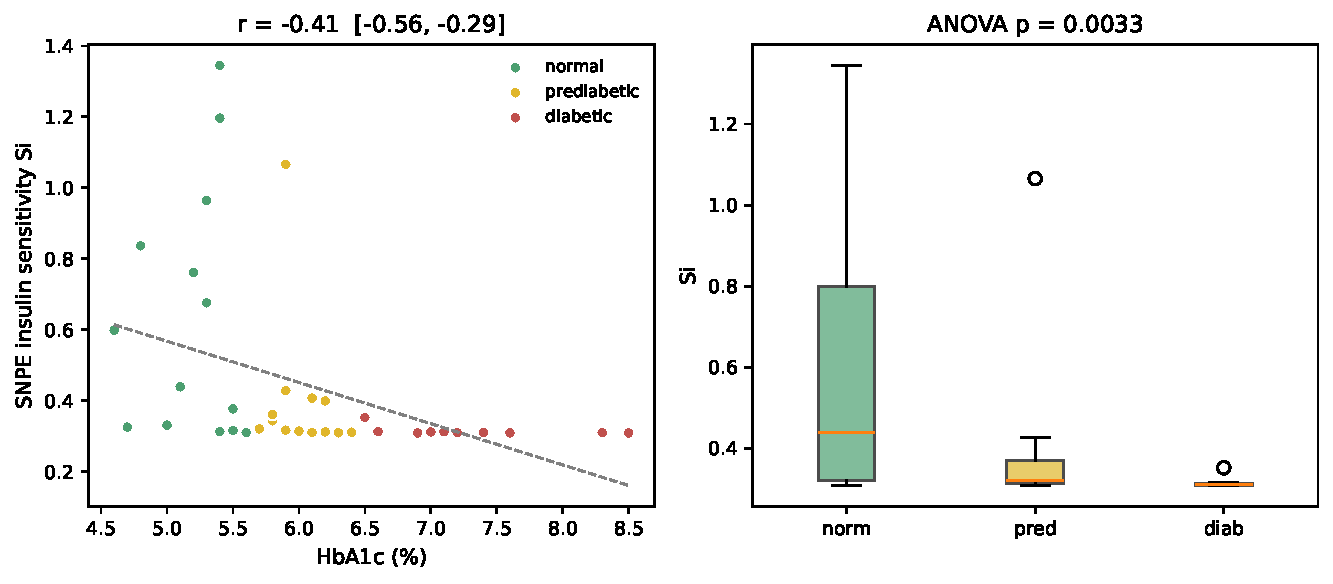
\includegraphics[width=0.95\columnwidth]{Figures/fig4_clinical_recovery}
\caption{CGMacros (n=45): gradient-inferred Si vs.\ HbA1c, colored by diagnostic group (left), and
Si distribution by group (right). Hall 2018 and ShanghaiT2DM results are reported alongside these
in Table~\ref{tab:clinical}.}
\label{fig:clinical}
\end{figure}

\begin{figure}[t]
\centering
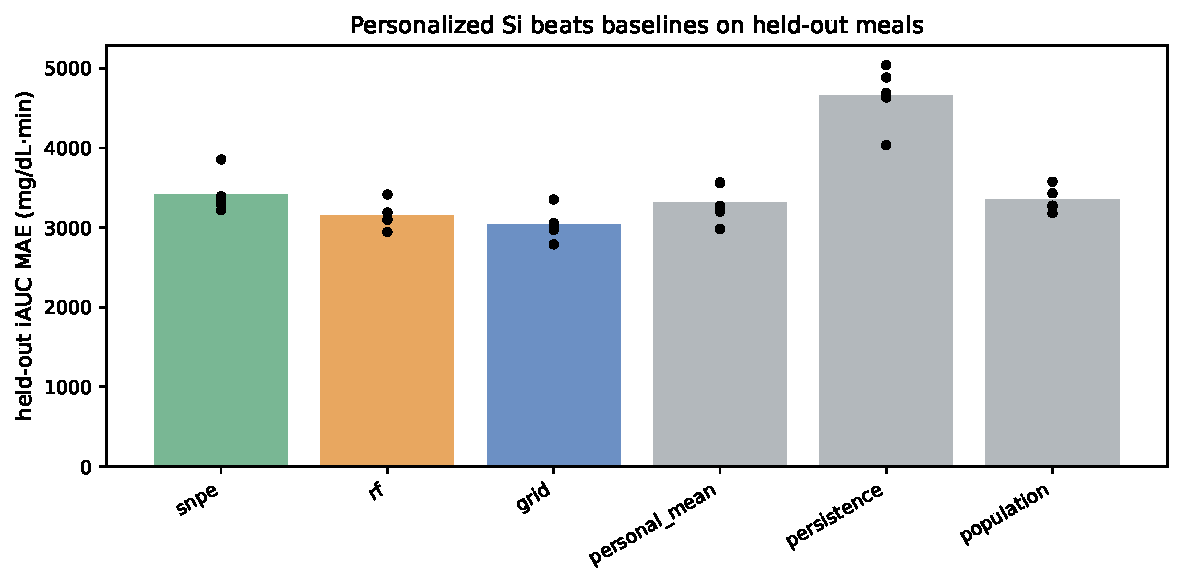
\includegraphics[width=0.95\columnwidth]{Figures/fig5_kfold_utility}
\caption{Held-out iAUC MAE by method (bars) with per-fold values (points) and personal-mean /
persistence baselines, aligned 5-fold protocol, CGMacros (n=45).}
\label{fig:kfold}
\end{figure}

\begin{figure}[t]
\centering
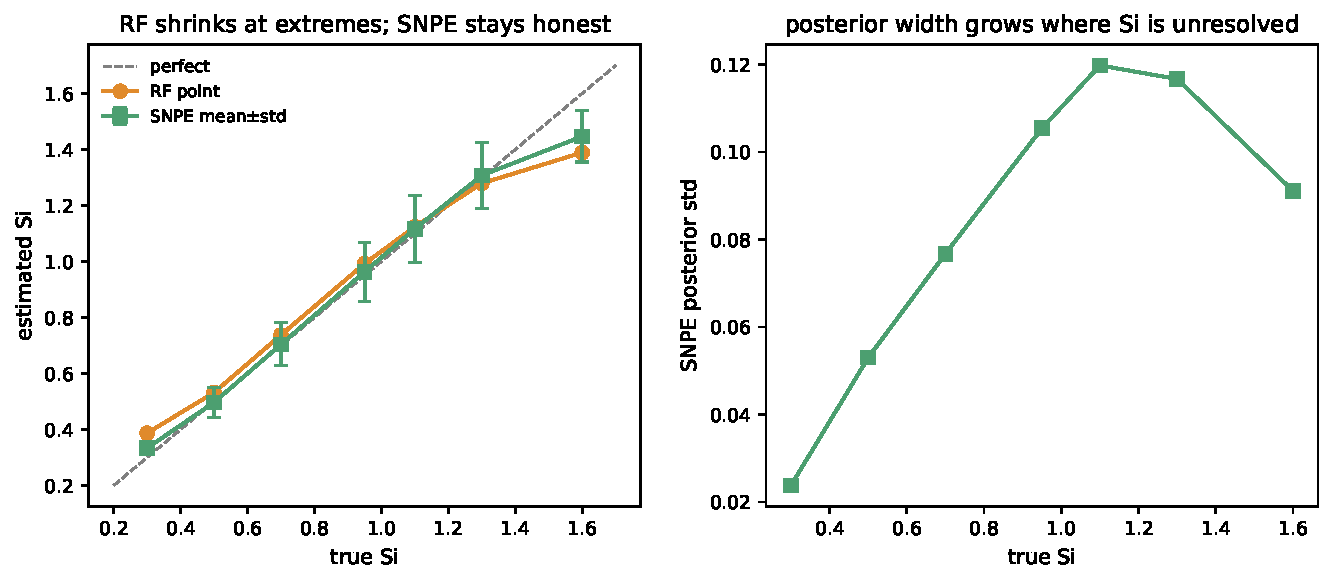
\includegraphics[width=0.95\columnwidth]{Figures/fig3_rf_vs_snpe}
\caption{Left: RF's point estimate shrinks toward the population mean at extreme true Si, while
SNPE's posterior mean tracks the true value with appropriately widening uncertainty. Right: SNPE
posterior width grows precisely where Si is least resolved by the data -- point estimation hides
non-identifiability that a calibrated posterior reveals.}
\label{fig:rfsnpe}
\end{figure}

\begin{figure}[t]
\centering
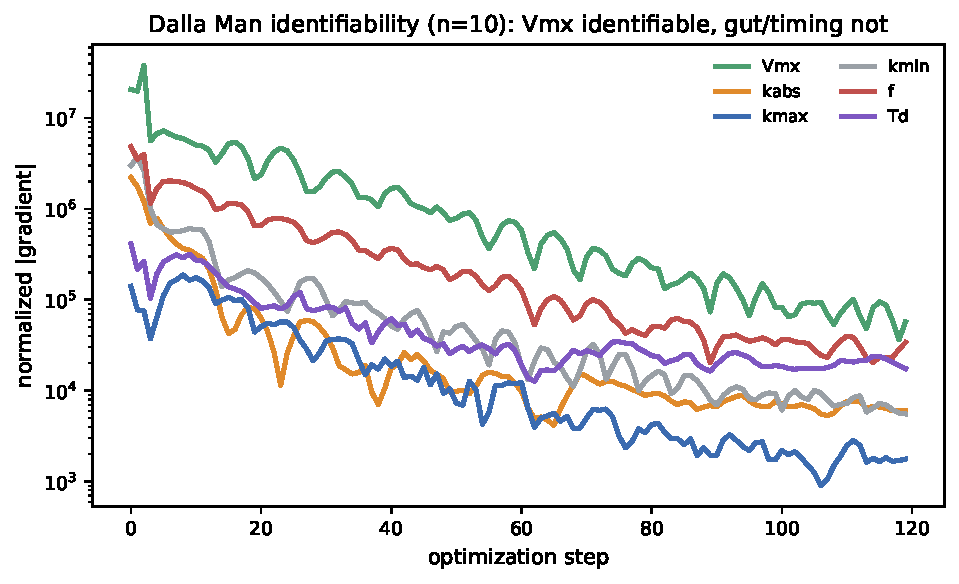
\includegraphics[width=0.95\columnwidth]{Figures/fig8_dalla_man_identifiability}
\caption{Gradient-norm identifiability replication on the Dalla Man-style model (representative
CGMacros subsample): the insulin-sensitivity-analog parameter $V_{mx}$ is identifiable; gut/timing
parameters are not -- the same structure as Figure~\ref{fig:gradnorm}, in a model with 11 states
instead of 3.}
\label{fig:dallaman}
\end{figure}

% References and End of Paper
% These lines must be placed at the end of your paper
\bibliography{aaai2027}

% The AAAI reproducibility checklist is submitted as a SEPARATE PDF in its own OpenReview field,
% not appended here -- see ReproducibilityChecklist.tex / ReproducibilityChecklist.pdf, compiled
% standalone via that file's \ifreproStandalone branch.

\end{document}
